\chapter*{Transformace obrazových signálů} \label{sec:transformace_obrazovych_signalu}

Při zpracování signálů, a to včetně signálů obrazových, se často uplatňují techniky opírající se o transformace signálu. V této kapitole se budeme problematice transformací signálu věnovat podrobněji. Nejprve se zaměříme na obecný pohled na transformace. Dále se pak budeme věnovat transformaci Fourierově, která mezi transformacemi zaujímá významné postavení a v praxi se často uplatňuje. Konečně uvedeme i některé další transformace. Transformací obecně rozumíme získání popisu signálu jako lineární kombinace funkcí jisté zvolené báze. Velmi často je vstupem (nebo naopak výstupem) transformace signál popsaný obrazovou funkcí přímo udávající intenzitu jasu v jednotlivých bodech obrazu. Nejprve ukážeme, že i tento nejběžnější způsob reprezentace obrazu lze interpretovat jako lineární kombinaci jistých bázových funkcí.

\section*{Báze $\delta$}

Uvažujme nejprve prostor $\mathscr{S}$ diskrétních signálů, kde definičním oborem signálů je množina $\Omega = \{0, 1, \dots, M-1\}$. V tomto prostoru uvažujme bázi

\begin{equation} \label{eq:2_1}
    \{\varphi_k(m) = \delta(k-m)\ | \ k, m = 0, 1, \dots, M-1\}.
\end{equation}

Je zřejmé, že tato báze je ortonormální. V prostoru $\mathcal{S}$ dále uvažujme signál popsaný funkcí $f(m)$ udávající intenzitu signálu v jednotlivých bodech. Ze vztahu \eqref{eq:1_2} víme, že každý signál je možné vyjádřit jako lineární kombinaci bázových funkcí. Je tedy

\begin{equation}
    f(m) = \sum\limits^{M-1}_{k=0} F(k)\delta(k-m).
\end{equation}

Hledejme nyní funkci $F(k)$. S využitím vztahu \eqref{eq:1_30} máme

\begin{equation} \label{eq:2_3}
    F(k) = \sum\limits^{M-1}_{k=0} F(m)\delta(k-m) = f(k), \, k = 0, 1, \dots, M-1.
\end{equation}

Na základě vztahu \eqref{eq:2_3} zjišťujeme, že pro bázi dle \eqref{eq:2_1} platí $F(k) = f(k)$. Tento závěr není překvapivý. Chtěli jsme zde pouze ukázat, že i běžný způsob praktické reprezentace diskrétního signálu pomocí $M$-tice $(f_0, f_1, \dots, f_{M-1})$ intenzit lze interpretovat z pohledu použití bázových funkcí. Analogicky můžeme postupovat také v prostoru spojitých signálů. Zvolme bázové jádro podle předpisu

\begin{equation} \label{eq:2_4}
    \varphi(u, x) = \delta(u-x).
\end{equation}

Opět je zřejmé, že takto zvolená báze je ortonormální. Uvažujme nyní v prostoru $\mathcal{S}$ spojitý signál $f(x)$ definovaný nad oblastí $\Omega$. Ze vztahu \eqref{eq:1_3} víme, že tento signál je možné zapsat ve tvaru lineární kombinace

\begin{equation} \label{eq:2_5}
    f(x) = \int\limits_U F(u) \delta(u-x) \,d u.
\end{equation}

Na základě vztahu \eqref{eq:1_33} pak máme

\begin{equation} \label{eq:2_6}
    F(u) = \int\limits_\Omega f(x) \delta(u-x) \,d x = f(u).
\end{equation}

Vztah \eqref{eq:2_6} ukazuje, že při volbě báze dle \eqref{eq:2_4} je hledaná funkce $F$ rovna přímo funkci $f$. I zde jsme chtěli ukázat, že i reprezentace signálu funkcí $f$ má interpretaci z pohledu bázových funkcí. Pro bázi dle vztahu \eqref{eq:2_1}, \eqref{eq:2_4} budeme v dalším textu používat názvu báze $\delta$.

\section*{Transformace signálu} \label{sec:transformace_signalu}

Mějme unitární prostor signálů. V tomto prostoru zvolme bázi. Transformací rozumíme pochod, kdy pro signál popsaný pomocí obrazové funkce (tedy jako lineární kombinace funkcí báze $\delta$) určujeme jeho popis pomocí zvolené báze. Zpětnou (inverzní) transformací pak nazýváme pochod opačný, kdy pro signál popsaný pomocí zvolené báze určujeme obrazovou funkci. Uvažujme nejprve diskrétní jednorozměrné signály. Transformací signálu $f(m)$ rozumíme nalezení funkce $F(k)$ ze vztahu \eqref{eq:1_2}, která signál reprezentuje s ohledem na zvolenou bázi $\{\varphi_k\}$. Je-li báze $\{\varphi_k\}$ ortonormální (což je výhodné a časté), pak lze pro výpočet koeficientů použít vztahu \eqref{eq:1_30}. Známe-li naopak funkci $F(k)$, pak lze obrazovou funkci $f(m)$ určit jako lineární kombinaci \eqref{eq:1_2}. Pro diskrérní dvojrozměrné signály je odpovídající zobecnění popsáno vztahy \eqref{eq:1_34}, \eqref{eq:1_4}.

Transformaci diskrétního dvojrozměrného signálu nazveme separabilní, jestliže platí

\begin{equation} \label{eq:2_7}
    \varphi_{k,l}(m, n) = \varphi_k(m)\varphi_l(n).
\end{equation}

Je-li transformace separabilní, pak ze vztahů \eqref{eq:1_34} a \eqref{eq:2_7} plyne

\begin{equation} \label{eq:2_8}
    F(k,l) = \sum\limits_{m=0}^{M-1}\left[\sum\limits_{n=0}^{N-1}f(m, n) \varphi_k^*(n)\right] \varphi_k^*(m).
\end{equation}

Vztah \eqref{eq:2_8} ukazuje, že jestliže je transformace separabilní, pak ji lze provádět odděleně po řádcích a po sloupcích bodů oblasti $\Omega$, nad níž je signál definován.

Předpokládejme nyní, že diskrétní dvojrozměrný signál je reprezentován jednorozměrným vektorem $\mathbf{f}$  (stačí zvolit pravidlo, podle kterého hodnoty $f(m,n)$ umisťujeme do jednorozměrného vektoru) a podobně předpokládejme, že i výsledek transformace je reprezentován jednorozměrným vektorem $\mathbf{F}$. Každý z těchto vektorů má $MN$ prvků. Ze vztahu \eqref{eq:1_3} vidíme, že každý prvek vektoru $\mathbf{F}$ je lineární kombinací prvků z $\mathbf{f}$. Lze tedy transformaci \eqref{eq:1_34} vyjádřit též maticovým zápisem

\begin{equation} \label{eq:2_9-10}
    \mathbf{F} = \mathbf{\Phi}\mathbf{f}, \quad \mathbf{f} = \mathbf{\Phi}^{-1}\mathbf{F},
\end{equation}

kde matice $\mathbf{\Phi}$ je rozměru $MN \times MN$. Poznamenejme, že je-li báze $\varphi_{k,l}(m,n)$ ortonormální, pak platí

\begin{equation} \label{eq:2_11}
    \mathbf{\Phi}^{-1} = \mathbf{\Phi}^{*\top}.
\end{equation}

Jestliže je transformace separabilní (vztah \eqref{eq:2_7}), pak lze nalézt maticový zápis, který je co do rozměru matic poněkud úspornější. Nechť je tentokrát signál před a po transformaci reprezentován maticemi $\mathbf{f}$ a $\mathbf{F}$, které jsou rozměru $M \times N$. Separabilní transformaci lze pak vyjádřit ve tvaru (praktický příklad uvedeme později v souvislosti s výpočtem Fourierovy transformace)

\begin{equation} \label{eq:2_12-13}
    \mathbf{F} = \mathbf{\Phi}_\mathsf{C} \mathbf{f} \mathbf{\Phi}_{\mathsf{R}}^{\top}, \quad \mathbf{f} = \mathbf{\Phi}_\mathsf{C}^{-1} \mathbf{F} \mathbf{\Phi}_{\mathsf{R}}^{\top^{-1}}.
\end{equation}

Podle očekávání lze analogicky postupovat také v prostoru spojitých signálů. Nechť $\mathscr{S}$ je takový prostor. V $\mathscr{S}$ zvolme bázové jádro $\varphi(u,x)$. Dále v $\mathscr{S}$ uvažujme signál $f(x)$. Transformací signálu rozumíme stanovení funkce $F(u)$, která uvažovaný signál reprezentuje s ohledem na zvolené bázové jádro. Splňuje-li bázové jádro podmínku ortonormality \eqref{eq:1_19}, pak lze pro výpočet této funkce použít vztahu \eqref{eq:1_33}. Známe-li naopak funkci $F(u)$, lze podle vztahu \eqref{eq:1_3} zapsat funkci $f(x)$ jako lineární kombinaci. Pro spojité dvojrozměrné signály lze obdobně uplatnit vztahy \eqref{eq:1_35}, \eqref{eq:1_5}.

\section*{Fourierova transformace}

Ústřední místo mezi transformacemi signálu zaujímá Fourierova transformace. V této podkapitole se zaměříme nejprve na spojitou Fourierovu transformaci, pak na transformaci diskrétní. Konečně uvedeme také příklad algoritmu výpočtu rychlé Fourierovy transformace.

\subsection*{Spojitá Fourierova transformace}

Uvažujme prostor signálů, kde oblast $\Omega$ definice signálu je dvojrozměrný euklidovský prostor E$^2$. Fourierovu transformaci obdržíme, jestliže bázové jádro volíme ve tvaru

\begin{equation} \label{eq:2_14}
    \varphi(u, v, x, y) = \exp \left[ j 2 \pi (ux + vy) \right].
\end{equation}

Ponecháváme na čtenáři, aby si ověřil, že uvedené bázové jádro je ortonormální - tj., že ve shodě se vztahem \eqref{eq:1_25} platí

\begin{equation} \label{eq:2_15}
    \int\limits_{-\infty}^{+\infty} \int\limits_{-\infty}^{+\infty} \exp \left[ j 2 \pi ( u_1 x + v_1 y ) \right] \exp \left[ - j 2 \pi ( u_2 x + v_2 y ) \right]\,dx\,dy = \delta(u_1 - u_2, v_1 - v_2).
\end{equation}

(Návod: Použijte vlastnost (1.48) Diracova impulzu.) Na základě vztahů \eqref{eq:1_35}, \eqref{eq:1_5} můžeme tedy pro spojitou Fourierovu transformaci dvojrozměrných signálů psát:

\begin{equation} \label{eq:2_16}
    F(u, v) = \int\limits_{-\infty}^{+\infty} \int\limits_{-\infty}^{+\infty} f(x, y) \exp \left[ - j 2 \pi ( u_2 x + v_2 y ) \right]\,dx\,dy = \int\limits_{-\infty}^{+\infty} \int\limits_{-\infty}^{+\infty} f(x, y) \left[ \cos 2 \pi (ux + vy) - j \sin 2 \pi (ux + vy) \right] \,dx \,dy,
\end{equation}

\begin{equation} \label{eq:2_17}
    f(x, y) = \int\limits_{-\infty}^{+\infty} \int\limits_{-\infty}^{+\infty} F(u, v) \exp \left[ j 2 \pi ( u x + v y ) \right]\,du\,dv = \int\limits_{-\infty}^{+\infty} \int\limits_{-\infty}^{+\infty} F(u, v) \left[ \cos 2 \pi (ux + vy) + j \sin 2 \pi (ux + vy) \right] \,du \,dv.
\end{equation}

Ze vztahu \eqref{eq:2_16} vyplývá, že obecně je $F(u, v)$ komplexní funkce. Rozepsáním na reálnou a imaginární složku máme

\begin{equation} \label{eq:2_18}
    F(u, v) = R(u, v) + \mathrm{j} I(u, v).
\end{equation}

Pro amplitudu $|F(u, v)|$ a fázový posuv $\Phi(u, v)$ pak platí

\begin{equation} \label{eq:2_19}
    |F(u, v)| = \sqrt{R^2(u, v) + I^2(u, v)}, \quad \Phi(u, v) = \arctan\left[ I(u, v) / R(u, v)\right].
\end{equation}

Hodnota $|F(u, v)|$ vyjadřuje, jak je frekvence $u$, $v$ obsažena v původní funkci $f(x, y)$. Funkce $|F(u, v)|^2$ se nazývá energetické spektrum signálu $f(x,y)$. Vztahy \eqref{eq:2_16}, \eqref{eq:2_17} provádí zobrazení komplexního signálového prostoru na sebe a jsou tedy operátorem nad tímto prostorem. Říkáme, že funkce $F(u, v)$ je Fourierovou transformací funkce $f(x, y)$ a funkce $f(x, y)$ je zpětnou (inverzní) Fourierovou transformací funkce $F(u, v)$. Tyto skutečnosti zapisujeme takto:

\begin{equation} \label{eq:2_20}
    F(u, v) = \mathscr{F}\{ f(x, y)\}, \quad f(x, y) = \mathscr{F}^{-1}\{F(u, v)\}.
\end{equation}

Poznamenejme ještě, že při zpracování obrazového signálu \textit{f}(\textit{x},\textit{y}) chápeme frekvenci jako „frekvenci délkovou`` - tj. kolik period se vejde na jednotku délky obrazu. Je dále zajímavé poukázat na souvislost Fourierovy transformace s Fourierovými řadami, které jsou dobře známé ze základního kurzu matematiky. Nechť \textit{f}(\textit{x},\textit{y}) je periodická funkce s periodou \textit{lx} ve směru osy \textit{x} a periodou \textit{ly} ve směru osy \textit{y}. Fourierovou řadou funkce \textit{f}(\textit{x},\textit{y}) pak nazýváme trigonometrickou řadu

\begin{equation} \label{eq:2_21}
    f(x, y) = \sum\limits_{m=-\infty}^{\infty} \sum\limits_{n=-\infty}^{\infty} c_{mn} \exp \left[ + \mathrm{j} 2 \pi \left( \frac{mx}{l_x} + \frac{ny}{l_y} \right) \right] = \sum\limits_{m=-\infty}^{\infty} \sum\limits_{n=-\infty}^{\infty} c_{mn} \left[ \cos 2 \pi \left( \frac{mx}{l_x} + \frac{ny}{l_y} \right) + \mathrm{j} \sin 2 \pi \left( \frac{mx}{l_x} + \frac{ny}{l_y} \right)\right],
\end{equation}
kde
\begin{equation} \label{eq:2_22}
    c_{mn} = \frac{1}{l_x l_y} \int\limits_{-l_x/2}^{l_x/2} \int\limits_{-l_y/2}^{l_y/2} f(x, y) \exp \left[ - \mathrm{j} 2 \pi \left( \frac{mx}{l_x} + \frac{ny}{l_y} \right) \right]\,dx\,dy.
\end{equation}

K přechodu od Fourierovy řady k Fourierově transformaci stačí obecnou (a tedy neperiodickou) funkci považovat za speciální případ funkce periodické, kdy je perioda nekonečně dlouhá, a dále vyjít z předpisu \eqref{eq:2_21} pro Fourierovu řadu: Uvažujme periodickou funkci \textit{f}(\textit{x},\textit{y}) s periodami $l_x$, $l_y$. Jestliže se periody $l_x$, $l_y$ prodlužují, pak se podle vztahu \eqref{eq:2_21} jednotlivé složky spektra navzájem přibližují až je nakonec při nekonečně dlouhých periodách vzdálenost mezi sousedními složkami spektra nekonečně malá. Diskrétní spektrum se tak změnilo ve spektrum spojité. Pro ilustraci spojité Fourierovy transformace uvedeme několik příkladů, jejichž výsledků později použijeme.

\textbf{Příklad 2.1.} Najdeme Fourierovu řadu pro funkci \textit{f}(\textit{x},\textit{y}), která je tvořena nekonečným polem Diracových impulzů, které se opakují ve vzdálenostech $\Delta$\textit{x}, $\Delta$\textit{y}. Uvedená funkce má tvar

\begin{figure}[th]
    \begin{center}
        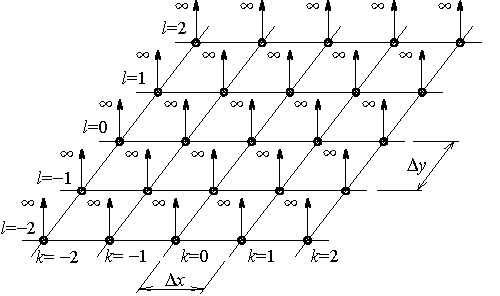
\includegraphics[scale=1.0]{02_transformace/images/img_2_1.pdf}
    \end{center}
    \caption{Pole Diracových impulzů.}
    \label{img:2_1}
\end{figure}

\begin{equation}
    f(x, y) = \sum\limits_{k=-\infty}^{\infty} \sum\limits_{l=-\infty}^{\infty} \delta( x - k\Delta x, y - l\Delta y ).\nonumber
\end{equation}

Funkce je vyobrazena na obr. \ref{img:2_1}. Podle vztahu \eqref{eq:2_22} máme

\begin{equation}
    c_{mn} = \frac{1}{\Delta x \Delta y} \int\limits_{-\Delta x/2}^{\Delta x/2} \int\limits_{-\Delta y/2}^{\Delta y/2} \delta(x - k\Delta x, y - l\Delta y) \exp \left[ - \mathrm{j} 2 \pi \left( \frac{mx}{\Delta x} + \frac{ny}{\Delta y} \right) \right]\,dx\,dy = \frac{1}{\Delta x \Delta y}.\nonumber
\end{equation}

Vztah pro $c_{mn}$ jsme obdrželi s uvážením skutečnosti, že integrujeme po délce jedné periody - v našem případě tedy od $-$$\Delta$\textit{x}/2 do $\Delta$\textit{x}/2  a od  $-$$\Delta$\textit{y}/ 2 do $\Delta$\textit{y}/2, kde $\delta$(\textit{x}$-$\textit{k}$\Delta$\textit{x}, \textit{y}$-$\textit{l}$\Delta$\textit{y}) nabývá nenulové hodnoty pouze pro \textit{k}=\textit{l}=0. Dále jsme využili vlastnost \eqref{eq:1_46} Diracova impulzu. Pro hledanou řadu pak podle vztahu \eqref{eq:2_21} vychází

\begin{equation}
    f(x, y) = \frac{1}{\Delta x \Delta y} \sum\limits_{m=-\infty}^{\infty} \sum\limits_{n=-\infty}^{\infty} \exp \left[ \mathrm{j} 2 \pi \left( \frac{mx}{\Delta x} + \frac{ny}{\Delta y} \right) \right].\nonumber
\end{equation}


\textbf{Příklad 2.2.} Nalezneme Fourierovu transformaci funkce $\delta_n$(\textit{x},\textit{y}) (odstavec 1.2.3). Na základě předpisu \eqref{eq:2_16} postupně dostáváme:

\begin{equation}
    F(u, v) = \int\limits_{-\infty}^{\infty} \int\limits_{-\infty}^{\infty} \delta_n(x, y) \exp \left[ - \mathrm{j} 2 \pi \left( ux + vy \right) \right]\,dx\,dy = n^2 \int\limits_{-1/2n}^{1/2n} \int\limits_{-1/2n}^{1/2n} \exp \left[ - \mathrm{j} 2 \pi \left( ux + vy \right)\right]\,dx\,dy = n^2 \int\limits_{-1/2n}^{1/2n} \exp\left[ - \mathrm{j} 2 \pi ux \right]\,dx \int\limits_{-1/2n}^{1/2n} \exp \left[ - \mathrm{j} 2 \pi vy \right]\,dy.\nonumber
\end{equation}
S využitím Eulerova vztahu  $e^{\mathrm{j}\varphi}$ = $\cos \varphi + \mathrm{j} \sin \varphi$ a po integraci pak vyjde

\begin{equation}
    F(u, v) = n^2 \frac{\sin (\pi u/ n)}{\pi u} \frac{\sin( \pi v / n )}{\pi v}.\nonumber
\end{equation}

Zavedeme funkci

\begin{equation}
    \mathrm{sinc} (u, v) = \frac{\sin (\pi u)}{\pi u} \frac{\sin( \pi v )}{\pi v}.\nonumber
\end{equation}

Pak vychází

\begin{equation} \label{eq:2_23}
    F(u, v) = \mathscr{F} \{ \delta_n(x, y) \} = \frac{\sin (\pi u/ n)}{\pi u} \frac{\sin( \pi v / n )}{\pi v} = \mathrm{sinc} \left( \frac{u}{n}, \frac{v}{n} \right).
\end{equation}

\begin{figure}[th]
    \begin{center}
        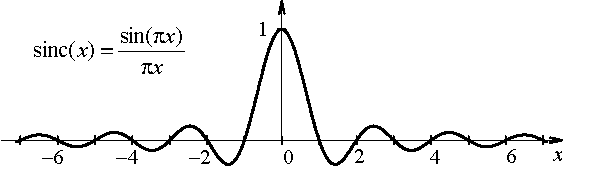
\includegraphics[scale=1.0]{02_transformace/images/img_2_2.pdf}
    \end{center}
    \caption{Funkce sinc(x).}
    \label{img:2_2}
\end{figure}

Konstatujeme, že obdélníkový impulz $\delta_n(x, y)$ má nekonečné spojité reálné frekvenční spektrum. Amplituta složek spektra je vyjádřena funkcí sinc(\textit{u}/\textit{n},\textit{v}/\textit{n}). Protože se s funkcí sinc budeme setkávat velmi často, uvádíme na obr. \ref{img:2_2} graf funkce sinc(\textit{x}).  $\cdot$

\noindent \textbf{Příklad 2.3.} Nalezneme Fourierovu transformaci Diracova impulzu $\delta$(\textit{x},\textit{y}). Využijeme výsledku z předchozího příkladu, kde položíme $n \rightarrow \infty$. Máme proto

\begin{equation}
    \mathscr{F} \{ \delta_n(x, y) \} = \lim\limits_{n \rightarrow \infty} \left[ \mathrm{sinc} \left( \frac{u}{n}, \frac{v}{n} \right) \right] = 1.
\end{equation}
Frekvenční spektrum Diracova impulzu $\delta$(\textit{x},\textit{y}) je opět spojité reálné a nekonečné. Amplituda všech složek spektra je konstantní a je rovna 1.

\noindent \textbf{Příklad 2.4.} Nalezneme Fourierovu transformaci funkce \textit{f}(\textit{x},\textit{y}), která je tvořena nekonečným polem Diracových impulzů opakujících se ve vzdálenostech $\Delta$\textit{x}, $\Delta$\textit{y}:

\begin{equation}
    f(x, y) = \sum\limits_{k=-\infty}^{\infty} \sum\limits_{k=-\infty}^{\infty} \delta(x - k\Delta x, y - l\Delta y).\nonumber
\end{equation}
Uvedená funkce je vyobrazena na obr. \ref{img:2_1}. V příkladě 2.1 jsme pro tuto funkci již našli Fourierovu řadu (funkce je periodická). Abychom obdrželi „pěkný`` výsledek, provedeme nyní místo Fourierovy transformace původní funkce transformaci jejího Fourierova rozvoje, který jsme obdrželi v příkladu 2.1. Z~příkladu 2.1 máme

\begin{equation}
    f(x, y) = \frac{1}{\Delta x \Delta y} \sum\limits_{m=-\infty}^{\infty} \sum\limits_{n=-\infty}^{\infty} \exp \left[ \mathrm{j} 2 \pi \left( \frac{mx}{\Delta x} + \frac{ny}{\Delta y} \right) \right].\nonumber
\end{equation}
Dosazením uvedeného vztahu do předpisu \eqref{eq:2_16} získáme

\begin{equation}
    F(u, v) = \int\limits_{-\infty}^{\infty} \int\limits_{-\infty}^{\infty} \frac{1}{\Delta x \Delta y} \sum\limits_{m=-\infty}^{\infty} \sum\limits_{n=-\infty}^{\infty} \exp \left[ \mathrm{j} 2 \pi \left( \frac{mx}{\Delta x} + \frac{ny}{\Delta y} \right) \right] \exp \left[ - \mathrm{j} 2 \pi (ux + vy) \right]\,dx\,dy.\nonumber
\end{equation}

\noindent Po záměně pořadí integrování a sumace a po úpravě dostaneme

\begin{equation}
    F(u, v) = \frac{1}{\Delta x \Delta y} \int\limits_{-\infty}^{\infty} \int\limits_{-\infty}^{\infty} \sum\limits_{m=-\infty}^{\infty} \sum\limits_{n=-\infty}^{\infty} \exp \left\{ \mathrm{j} 2 \pi \left[ \left( u - \frac{m}{\Delta x} \right) + \left( v - \frac{n}{\Delta y} \right) \right] \right\} \,dx\,dy.\nonumber
\end{equation}
S uvážením vlastnosti \eqref{eq:1_48} Diracova impuzu pak konečně obdržíme vztah

\begin{equation}
    F(u, v) = \frac{1}{\Delta x \Delta y} \sum\limits_{m=-\infty}^{\infty} \sum\limits_{n=-\infty}^{\infty} \delta \left( u - \frac{m}{\Delta x}, v - \frac{n}{\Delta y} \right).\nonumber
\end{equation}

\noindent Vidíme, že Fourierovým obrazem nekonečného pole Diracových impulzů vzdálených vzájemně o $\Delta$\textit{x}, $\Delta$\textit{y} je opět nekonečné pole Diracových impulzů, kde jsou impulzy vzájemně vzdáleny o 1/$\Delta$\textit{x}, 1/$\Delta$\textit{y}.

\noindent \textbf{Příklad 2.5.} Ukažte, že Fourierovou transformací funkce cos(2$\pi$\textit{ax}) je funkce $[$$\delta$(\textit{u}$-$\textit{a})+$\delta$(\textit{u}+\textit{a})$]$/2. Provedení příkladu ponecháváme čtenáři jako cvičení. Návod: použijte vztahu $\cos \varphi = (e^{\mathrm{j}\varphi} + e^{-\mathrm{j}\varphi})/2$ a dále použijte vlastnosti \eqref{eq:1_48} Diracova impulzu. Z příkladu vidíme, že spektrum funkce cos(2$\pi$\textit{ax}) obsahuje pouze složky \textit{u} = \textit{a}, \textit{u} = $-$\textit{a}. Takový výsledek jsme ovšem jistě intuitivně očekávali.

\subsection*{Vlastnosti spojité Fourierovy transformace}

V tomto odstavci uvedeme několik vlastností Fourierovy transformace, které se ve zpracování obrazu často uplatňují. Protože důkazy uvedených vlastností jsou vesměs jednoduché, ponecháváme je čtenáři jako cvičení (zpravidla však uvádíme stručný návod, jak při důkazu postupovat). Ve shodě s dříve používaným značením je i zde $F(u, v) = \mathscr{F}\{f(x, y)\}$ Fourierův obraz funkce $f(x, y)$, $G(u, v) = \mathscr{F}\{g(x, y)\}$ Fourierův obraz funkce \textit{g}(\textit{x},\textit{y}); \textit{a}, \textit{b} jsou čísla. Obecně mohou být funkce \textit{f}(\textit{x},\textit{y}), \textit{g}(\textit{x},\textit{y}) i čísla \textit{a},\textit{b} komplexní.

\noindent \textbf{a) Linearita:} \textbf{F}\{\textit{af}(\textit{x},\textit{y})+\textit{bg}(\textit{x},\textit{y})\} = \textit{a}\textbf{F}\{\textit{f}(\textit{x},\textit{y})\} + \textit{b}\textbf{F}\{\textit{g}(\textit{x},\textit{y})\} = \textit{aF}(\textit{u},\textit{v}) + \textit{bG}(\textit{u},\textit{v}). \eqref{eq:2_24}

\begin{equation} \label{eq:2_24}
    \mathscr{F}\{af(x, y) + bg(x, y)\} = a\mathscr{F}\{f(x,y)\} + b\mathscr{F}\{g(x, y)\} = aF(u, v) + bG(u, v).
\end{equation}

\noindent K důkazu této vlastnosti použijte předpis \eqref{eq:2_16} pro Fourierovu transformaci. Dále již vlastnost přímo vyplývá z vlastností integrování.

\noindent \textbf{b) Měřítko:} Nechť $\alpha$,$\beta$ jsou reálná čísla. Pak platí

\begin{equation} \label{eq:2_25}
    \mathscr{F}\{f ( \alpha x, \beta y)\} = F( u / \alpha, v / \beta) / | \alpha \beta |.
\end{equation}

\noindent K důkazu této vlastnosti vyjděte z předpisu pro Fourierovu transformaci a zaveďte transformaci proměnných $x' = \alpha x$, $y' = \beta y$.

\noindent \textbf{c) Posuv:}

\begin{equation} \label{eq:2_26a}
    \mathscr{F}\{f(x - x_o, y - y_o)\} = F(u, v) \exp \left[ - \mathrm{j} 2 \pi (ux_o + vy_o)\right].
\end{equation}

\noindent K důkazu této vlastnosti vyjděte z předpisu pro Fourierovu transformaci a zaveďte transformaci proměnných $x' = x - x_o, y' = y - y_o$. Podobnou vlastnost lze nalézt také ve frekvenční doméně:

\begin{equation} \label{eq:2_26b}
    \mathscr{F}^{-1}\{F(u - u_o, v - v_o)\} = f(x, y) \exp \left[ \mathrm{j} 2 \pi (u_o x + v_o y)\right].
\end{equation}
Vlastnost \eqref{eq:2_26b} bývá nazývána modulací. Ponecháváme na čtenáři, aby promyslel oprávněnost tohoto názvu.

\noindent \textbf{d) Reflexe:} \textbf{F}\{\textit{f}($-$\textit{x},\textit{y})\} = \textit{F}($-$\textit{u},\textit{v}),     \textbf{F}\{\textit{f}(\textit{x},$-$\textit{y})\} = \textit{F}(\textit{u},$-$\textit{v}),     \textbf{F}\{\textit{f}($-$\textit{x},$-$\textit{y})\} = \textit{F}($-$\textit{u},$-$\textit{v}) (2.27a)

\begin{equation} \label{eq:2_27a}
    \mathscr{F}\{f(-x, y)\} = F(-u, v), \quad \mathscr{F}\{f(x, -y)\} = F(u, - v), \quad \mathscr{F}\{f( -x, -y)\} = {F}( -u, -v)
\end{equation}
a také
\begin{equation} \label{eq:2_27b}
    \mathscr{F}\{f^*( -x, -y)\} = F^*(u, v),
\end{equation}
kde $^*$ označuje komplexně sdruženou veličinu. K důkazu vlastností \eqref{eq:2_27a} opět postačí substituce $x' = -x$, $y' = -y$. K důkazu vlastnosti \eqref{eq:2_27b} použijte předpisu \eqref{eq:2_16} pro \textit{F}(\textit{u},\textit{v}), proveďte komplexní sdružení a výsledek dále upravte.

\noindent \textbf{e) Konvoluční teorém:}

\begin{equation} \label{eq:2_28a}
    \mathscr{F}\{f(x, y) * g(x, y)\} = F(u, v) G(u, v),
\end{equation}

\begin{equation} \label{eq:2_28b}
    \mathscr{F}\{f(x, y) g(x, y)\} = F(u, v) * G(u, v).
\end{equation}
Vlastnost \eqref{eq:2_28a}, \eqref{eq:2_28b} je významná a později ji mnohokrát využijeme. Říká, že Fourierovým obrazem konvoluce funkcí \textit{f}, \textit{g} je součin Fourierových obrazů \textit{F}, \textit{G} obou funkcí. Podobně je Fourierovým obrazem součinu funkcí \textit{f}, \textit{g} konvoluce Fourierových obrazů \textit{F}, \textit{G} obou funkcí. S ohledem na mimořádný význam uvedených tvrzení provedeme tentokrát i důkaz.

\noindent \textbf{Důkaz.} Dokážeme vlastnost \eqref{eq:2_28a}. Důkaz druhé vlastnosti lze provést obdobně. Víme, že konvoluce funkcí je definována předpisem

\begin{equation}
    f(x, y) * g(x, y) = \int\limits_{-\infty}^{\infty} \int\limits_{-\infty}^{\infty} f(a, b) g( x - a, y - b)\,da\,db.\nonumber
\end{equation}
Pro Fourierovu transformaci konvoluce pak podle předpisu \eqref{eq:2_16} máme

\begin{equation}
    \mathscr{F}\{ f(x, y) * g(x, y) \} = \int\limits_{-\infty}^{\infty} \int\limits_{-\infty}^{\infty} \left[ \int\limits_{-\infty}^{\infty} \int\limits_{-\infty}^{\infty} f(a, b) g( x - a, y - b)\,da\,db \right] \exp \left[ - \mathrm{j} 2 \pi (ux + vy) \right]\,dx\,dy.\nonumber
\end{equation}
Záměnou pořadí integrace dostáváme

\begin{equation}
    \mathscr{F}\{ f(x, y) * g(x, y) \} = \int\limits_{-\infty}^{\infty} \int\limits_{-\infty}^{\infty} f(a, b) \left[ \int\limits_{-\infty}^{\infty} \int\limits_{-\infty}^{\infty} g( x - a, y - b) \exp \left[ - \mathrm{j} 2 \pi (ux + vy) \right]\,dx\,dy \right]\,da\,db.\nonumber
\end{equation}
Uplatněním vlastnosti \eqref{eq:2_26a} získáme

\begin{equation}
    \mathscr{F}\{ f(x, y) * g(x, y) \} = \int\limits_{-\infty}^{\infty} \int\limits_{-\infty}^{\infty} f(a, b) G(u, v) \exp \left[ - \mathrm{j} 2 \pi (ua + vb) \right]\,da\,db.\nonumber
\end{equation}
Tento vztah lze pak již konečně upravit na tvar

\begin{equation}
    \mathscr{F}\{ f(x, y) * g(x, y) \} = G(u, v)  \int\limits_{-\infty}^{\infty} \int\limits_{-\infty}^{\infty} f(a, b) \exp \left[ - \mathrm{j} 2 \pi (ua + vb) \right]\,da\,db = F(u, v)G(u, v).\nonumber
\end{equation}

\textbf{f) Parsevalův teorém: }Předpokládejme, že obecně jsou funkce \textit{f}(\textit{x},\textit{y}), \textit{g}(\textit{x},\textit{y}) komplexní a použijme symbolu $^*$ pro označení funkce komplexně sdružené. Parsevalův teorém tvrdí:

\begin{equation} \label{eq:2_29}
    \int\limits_{-\infty}^{\infty} \int\limits_{-\infty}^{\infty} f(x, y) g^*(x, y)\,dx\,dy = \int\limits_{-\infty}^{\infty} \int\limits_{-\infty}^{\infty} F(u, v) G^*(u, v)\,du\,dv.
\end{equation}
Ve speciálním případě, kdy je  \textit{f}(\textit{x},\textit{y}) = \textit{g}(\textit{x},\textit{y}),  přechází uvedený výraz na tvar

\begin{equation} \label{eq:2_30}
    \int\limits_{-\infty}^{\infty} \int\limits_{-\infty}^{\infty} |f(x, y)|^2\,dx\,dy = \int\limits_{-\infty}^{\infty} \int\limits_{-\infty}^{\infty} |F(u, v)|^2 \,du\,dv.
\end{equation}
Výraz na levé straně vztahu \eqref{eq:2_30} může být interpretován jako celkový výkon signálu \textit{f}(\textit{x},\textit{y}). Výraz $|F(u, v)|^2$ má proto význam výkonového spektra signálu \textit{f}(\textit{x},\textit{y}).

\noindent \textbf{g) Korelační teorém:} Opět předpokládejme, že obecně jsou funkce \textit{f}(\textit{x},\textit{y}), \textit{g}(\textit{x},\textit{y}) komplexní. Křížová korelace $R_{fg}$ a autokorelace $R_{ff}$ deterministických funkcí \textit{f}(\textit{x},\textit{y}) a \textit{g}(\textit{x},\textit{y}) jsou definovány pomocí vztahů

\begin{equation} \label{eq:2_31}
    R_{fg} (a, b) = \int\limits_{-\infty}^{\infty} \int\limits_{-\infty}^{\infty} f^*(x - a, y - b) g(x, y)\,dx\,dy,
\end{equation}

\begin{equation} \label{eq:2_32}
    R_{ff} (a, b) = \int\limits_{-\infty}^{\infty} \int\limits_{-\infty}^{\infty} f^*(x - a, y - b) f(x, y)\,dx\,dy = \int\limits_{-\infty}^{\infty} \int\limits_{-\infty}^{\infty} f(x + a, y + b) f^*(x, y)\,dx\,dy,
\end{equation}
Ne náhodou uvedené vztahy připomínají čtenáři vztah pro konvoluci. Skutečně, jediný rozdíl je ve znaménku členu (\textit{x}$-$\textit{a}, \textit{y}$-$\textit{b}). Také tvrzení korelačního teorému koresponduje s tvrzením teorému konvolučního. Korelační teorém totiž tvrdí:

\begin{equation} \label{eq:2_33}
    \mathscr{F}\{R_{fg}\} = F^*(u, v) G(u, v),
\end{equation}

\begin{equation} \label{eq:2_34}
    \mathscr{F}\{R_{ff}\} = F^*(u, v) F(u, v) = |F(u, v)|^2.
\end{equation}
Důkaz vztahu \eqref{eq:2_33} lze provést podobně jako u konvolučního teorému. Vztah \eqref{eq:2_34} vyplývá ze vztahu \eqref{eq:2_33}.

\noindent \textbf{h) Derivace: }Pro Fourierův obraz derivace funkce platí vztahy

\begin{equation} \label{eq:2_35}
    \mathscr{F}\left\{\frac{\partial f(x, y)}{\partial x}\right\} = \mathrm{j} 2 \pi u F(u, v), \quad \mathscr{F}\left\{\frac{\partial f(x, y)}{\partial y}\right\} = \mathrm{j} 2 \pi v F(u, v)
\end{equation}

\noindent K důkazu této vlastnosti stačí vyjít z definice Fourierovy transformace a použít integrace per partes. Při tom předpokládáme, že platí  \textit{f}($-$$\infty$,\textit{y}) = \textit{f}($\infty$,\textit{y}) = \textit{f}(\textit{x},$-$$\infty$) = \textit{f}(\textit{x},$\infty$) = 0.  Analogicky lze také odvodit např. vztah pro Fourierův obraz laplaciánu funkce. Dostaneme

\begin{equation} \label{eq:2_36}
    \mathscr{F}\left\{\frac{\partial^2 f(x, y)}{\partial x^2} + \frac{\partial^2 f(x, y)}{\partial y^2} \right\} = - 4 \pi^2 ( u^2 + v^2 ) F(u, v)
\end{equation}

\subsection*{Diskrétní Fourierova transformace}

\noindent Uvažujme prostor signálů, kde je oblast $\Omega$, nad níž jsou signály definovány, tvořena množinou bodů, které indexujeme pomocí dvojice indexů \textit{m} = 0, 1,\dots, \textit{M}$-$1,  \textit{n} = 0, 1, \dots, \textit{N}$-$1. Diskrétní Fourierovu transformaci v~tomto prostoru obdržíme, jestliže bázi volíme ve tvaru

\begin{equation} \label{eq:2_37}
    \varphi_{k,l}(m, n) = \frac{1}{\sqrt{MN}} \exp \left[ \mathrm{j} 2 \pi \left( \frac{mk}{M} + \frac{nl}{N} \right) \right] \, k = 0, 1, \dots, M-1, \,l = 0, 1, \dots, N-1.
\end{equation}
Opět ponecháváme na čtenáři, aby ověřil, že takto zvolená báze je ortonormální - tj., že platí

\begin{equation} \label{eq:2_38}
    \frac{1}{\sqrt{MN}} \sum\limits_{m=0}^{M-1} \sum\limits_{n=0}^{N-1} \exp \left[ \mathrm{j} 2 \pi \left( \frac{mk_1}{M} + \frac{nl_1}{N} \right) \right] \exp \left[ - \mathrm{j} 2 \pi \left( \frac{mk_2}{M} + \frac{nl_2}{N} \right) \right] = \delta( k_1 - k_2, l_1 - l_2 ).
\end{equation}
Podle vztahu \eqref{eq:1_34} pak pro diskrétní Fourierovu transformaci platí

\begin{equation} \label{eq:2_39}
    F(k, l) = \frac{1}{\sqrt{MN}} \sum\limits_{m=0}^{M-1} \sum\limits_{n=0}^{N-1} f(m, n) \exp \left[ - \mathrm{j} 2 \pi \left( \frac{mk}{M} + \frac{nl}{N} \right) \right],\, k = 0, 1, \dots, M-1,\, l = 0, 1, \dots, N-1.
\end{equation}
V souladu se vztahem \eqref{eq:1_4} pro zpětnou Fourierovu transformaci dostáváme

\begin{equation} \label{eq:2_40}
    f(m, n) = \frac{1}{\sqrt{MN}} \sum\limits_{m=0}^{M-1} \sum\limits_{n=0}^{N-1} F(k, l) \exp \left[ \mathrm{j} 2 \pi \left( \frac{mk}{M} + \frac{nl}{N} \right) \right].
\end{equation}

\noindent Předpokládejme nyní, že signál je reprezentován maticí $\mathbf{f}$ a jeho Fourierův obraz maticí \textbf{F}. Obě matice mají rozměr \textit{M}$\times$\textit{N}. Protože Fourierova transformace je separabilní, lze ji zapsat podle vztahu \eqref{eq:2_12-13} ve tvaru

\begin{equation} \label{eq:2_41}
    \mathbf{F} = \mathbf{\Phi}_{\mathsf{C}} \mathbf{f} \mathbf{\Phi}_{\mathsf{R}}.
\end{equation}
Zaveďme označení

\begin{equation} \label{eq:2_42}
    W_M = \exp \left[ \frac{ - \mathrm{j} 2 \pi}{M} \right].
\end{equation}
Pro matice $\mathbf{\Phi}_{\mathsf{R}}$, $\mathbf{\Phi}_{\mathsf{C}}$ pak platí

\begin{equation} \label{eq:2_43} 
    \mathbf{\Phi}_{\mathsf{R}} = \frac{1}{\sqrt{N}} \left[
    \begin{array}{ccccc}
    W_N^0 & W_N^0 & W_N^0 & \cdots & W_N^0\\
    W_N^0 & W_N^1 & W_N^2 & \cdots & W_N^{N-1} \\
    W_N^0 & W_N^2 & W_N^4 & \cdots & W_N^{N-1} \\
    \cdots & \cdots & \cdots & \ddots & \cdots \\
    W_N^0 & W_N^{N-1} & W_N^{2(N-1)} & \cdots & W_N^{(N-1)^2} \\
    \end{array}\right],
\end{equation} 

\begin{equation} \label{eq:2_44} 
    \mathbf{\Phi}_{\mathsf{C}} = \frac{1}{\sqrt{M}} \left[
    \begin{array}{ccccc}
    W_M^0 & W_M^0 & W_M^0 & \cdots & W_M^0\\
    W_M^0 & W_M^1 & W_M^2 & \cdots & W_M^{M-1} \\
    W_M^0 & W_M^2 & W_M^4 & \cdots & W_M^{M-1} \\
    \cdots & \cdots & \cdots & \ddots & \cdots \\
    W_M^0 & W_M^{M-1} & W_M^{2(M-1)} & \cdots & W_M^{(M-1)^2} \\
    \end{array}\right].
\end{equation} 
Zpětnou Fourierovu transformaci lze pak zapsat maticovým vztahem

\begin{equation} \label{eq:2_45}
    \mathbf{f} = \mathbf{\Phi}_{\mathsf{C}}^* \mathbf{F} \mathbf{\Phi}_{\mathsf{R}}^*.
\end{equation}
kde * znamená komplexně sdružené matice.

\subsection*{Vlastnosti diskrétní Fourierovy transformace}

V tomto odstavci uvedeme několik významnějších vlastností diskrétní Fourierovy transformace. Jistě nepřekvapí, že většina z nich koresponduje s vlastnostmi Fourierovy transformace spojité. Vlastnosti proto uvedeme pouze ve stručném přehledu. Předpokládejme, že \textit{f}(\textit{m},\textit{n}), \textit{g}(\textit{m},\textit{n}) jsou diskrétní signály, \textit{F}(\textit{k},\textit{l}), \textit{G}(\textit{k},\textit{l}) jsou Fourierovy obrazy těchto signálů, \textit{a},\textit{b} jsou čísla (obecně komplexní). Vlastnosti diskrétní Fourierovy transformace pak můžeme formulovat takto:

\noindent \textbf{a) Linearita:}

\begin{equation} \label{eq:2_46}
    \mathscr{F}\{af(m, n) + bg(m, n)\} = a\mathscr{F}\{f(m, n)\} + b\mathscr{F}\{g(m, n)\} = aF(k, l) + bG(k, l).
\end{equation}

\noindent \textbf{b) Periodicita:} Ve výrazu \eqref{eq:2_39} pro Fourierovu transformaci jsme předpokládali, že \textit{k},\textit{l} jsou z rozsahu \textit{k} = 0, 1, 2, \dots, \textit{M}$-$1  a  \textit{l} = 0, 1, 2, \dots, \textit{N}$-$1. Pokud bychom se pokoušeli vypočítat hodnoty Fourierova obrazu pro  \textit{k}, \textit{l}  mimo uvedené meze, pak analýzou vztahu \eqref{eq:2_39} zjistíme, že platí

\begin{equation} \label{eq:2_47}
    F(k, -l) = F(k, N-l), \, F(-k, l) = F(M-k, l), \, F(-k, -l) = F(M-k, N-l),
\end{equation}

\begin{equation} \label{eq:2_48}
    F(\alpha M + k, \beta N + l) = F(k, l), \quad \alpha, \beta = 0, \pm 1, \pm 2, \dots.
\end{equation}
Podobně také z předpisu \eqref{eq:2_40} pro zpětnou transformaci vychází

\begin{equation} \label{eq:2_49}
    f(-m, n) = f(M -m, n), \, f(m, -n) = f(m, N-n), \, f(-m, -n) = f(M-m, N-n),
\end{equation}

\begin{equation} \label{eq:2_50}
    f(\alpha M+m, \beta N+n) = f(m, n), \quad \alpha, \beta = 0, \pm 1, \pm 2, \dots.
\end{equation}
Uvedené vlastnosti vyplývají z periodicity exponenciálního členu ve výrazech \eqref{eq:2_39}, \eqref{eq:2_40}.

\noindent \textbf{c) Kruhový posuv: }Nechť \textit{f}(\textit{m},\textit{n}) je periodická funkce s periodou \textit{M},\textit{N}. Pro Fourierovu transformaci funkce \textit{f}(\textit{m}$-$\textit{m}$_0$,\textit{n}$-$\textit{n}$_0$) platí

\begin{equation} \label{eq:2_51a}
    \mathscr{F}\{ f(m - m_0, n - n_0)\} = F(k, l) \exp \left[ - \mathrm{j} 2 \pi \left( \frac{m_0 k}{M} + \frac{n_0 l}{N}\right) \right].
\end{equation}
Podobnou vlastnost lze nalézt také ve frekvenční doméně:

\begin{equation} \label{eq:2_51b}
    \mathscr{F}^{-1}\{ F(k - k_0, l - l_0)\} = f(m, n) \exp \left[ \mathrm{j} 2 \pi \left( \frac{m k_0}{M} + \frac{n l_0}{N}\right) \right].
\end{equation}
Poznamenejme, že předpoklad periodicity funkce \textit{f}(\textit{m},\textit{n}) jsme zde zavedli k tomu, aby funkce \textit{f}(\textit{m}$-$\textit{m}$_0$,\textit{n}$-$\textit{n}$_0$)  byla definována na celé oblasti  \textit{m} = 0, 1, \dots, \textit{M}$-$1;  \textit{n} = 0, 1, \dots, \textit{N}$-$1 pro každé \textit{m}$_0$, \textit{n}$_0$.

\noindent \textbf{d) Komplexně sdružená hodnota: }Je-li funkce \textit{f}(\textit{m},\textit{n}) reálná, pak platí

\begin{equation} \label{eq:2_52}
    F(\alpha M-k, \beta N-l) = F^*(k, l), \quad \alpha, \beta = 1, 2, \dots \, .
\end{equation}
Vlastnost snadno dokážeme, jestliže levou i pravou stranu rovnice \eqref{eq:2_52} rozepíšeme podle vztahu \eqref{eq:2_39}. Pro praktický výpočet diskrétní Fourierovy transformace reálných signálů má vlastnost velký význam. S jejím využitím postačí hodnoty \textit{F}(\textit{k},\textit{l}) počítat přibližně v polovině bodů.

\noindent \textbf{e) Konvoluční teorém: }Podobně jako pro spojitou Fourierovu transformaci platí i pro transformaci diskrétní, že Fourierova transformace konvoluce funkcí v prostorové doméně je součinem Fourierových obrazů funkcí v doméně frekvenční a naopak součinu v prostorové doméně odpovídá konvoluce v doméně frekvenční. Konvoluce se v tomto případě uvažuje cyklická. Je tedy

\begin{equation} \label{eq:2_53a}
    \mathscr{F}\{ f(m, n) * g(m, n) \} = \frac{1}{\sqrt{MN}} F(k, l) G(k, l),
\end{equation}

\begin{equation} \label{eq:2_53b}
    \mathscr{F}\{ f(m, n) g(m, n) \} = \frac{1}{\sqrt{MN}} F(k, l) * G(k, l),
\end{equation}

\noindent \textbf{f) Korelační teorém: }Definujme nejprve křížovou korelaci $R_{fg}$ a autokorelaci $R_{ff}$ deterministických diskrétních funkcí \textit{f}(\textit{m},\textit{n}), \textit{g}(\textit{m},\textit{n}):

\begin{equation} \label{eq:2_54}
    R_{fg}(m, n) = \frac{1}{MN} \sum\limits_{r=0}^{M-1} \sum\limits_{s=0}^{N-1} f^*(r - m, s - n) g(r, s),
\end{equation}

\begin{equation} \label{eq:2_55}
    R_{ff}(m, n) = \frac{1}{MN} \sum\limits_{r=0}^{M-1} \sum\limits_{s=0}^{N-1} f^*(r - m, s - n) f(r, s) = \frac{1}{MN} \sum\limits_{r=0}^{M-1} \sum\limits_{s=0}^{N-1} f(r + m, s + n) f^*(r, s).
\end{equation}
Korelační teorém tvrdí:

\begin{equation} \label{eq:2_56}
    \mathscr{F}\{ R_{FF}(m, n) \} = \frac{1}{\sqrt{MN}} F^*(k, l) G(k, l),
\end{equation}

\begin{equation} \label{eq:2_57}
    \mathscr{F}\{ R_{FF}(m, n) \} = \frac{1}{\sqrt{MN}} F^*(k, l) F(k, l) = \frac{1}{\sqrt{MN}} |F(k, l)|^2.
\end{equation}
Poznamenejme, že podobně jako u konvoluce se i korelace a autokorelace uvažují cyklické (nebo se předpokládá, že funkce \textit{f}(\textit{m},\textit{n}), \textit{g}(\textit{m},\textit{n}) jsou periodické).

\noindent \textbf{g) Parsevalův teorém: }Předpokládejme, že obecně jsou signály \textit{f}(\textit{x},\textit{y}), \textit{g}(\textit{x},\textit{y}) komplexní a použijme symbolu * pro označení komplexně sdružené funkce. Parsevalův teorém tvrdí:

\begin{equation} \label{eq:2_58}
    \sum\limits_{m=0}^{M-1} \sum\limits_{n=0}^{N-1} f(m, n) g^*(m, n) = \sum\limits_{k=0}^{M-1} \sum\limits_{l=0}^{N-1} F(k, l)G^*(k, l).
\end{equation}
Ve speciálním případě, kdy  \textit{f}(\textit{x},\textit{y}) = \textit{g}(\textit{x},\textit{y}), přechází uvedený výraz na tvar

\begin{equation} \label{eq:2_59}
    \sum\limits_{m=0}^{M-1} \sum\limits_{n=0}^{N-1} |f(m, n)|^2 = \sum\limits_{k=0}^{M-1} \sum\limits_{l=0}^{N-1} |F(k, l)|^2.
\end{equation}

%\subsection*{Rychlá Fourierova transformace}

%\noindent Ze vztahu \eqref{GrindEQ__2_39_} vidíme, že algoritmus výpočtu dvojrozměrné diskrétní Fourierovy transformace může ve své naivní podobě dosáhnout časové složitosti řádově \textit{M}2\textit{N}2 operací. Při tak vysoké složitosti by možnosti praktického použití Fourierovy transformace při číslicovém zpracování dvojrozměrných signálů byly velmi omezené. Naštěstí však byly nalezeny algoritmy, jejichž časová složitost je podstatně nižší. Ukážeme zde podrobněji jeden z nich. Efektivnost algoritmu je založena na využití techniky dělení na podproblémy poloviční velikosti, s níž se při konstrukci efektivních algoritmů setkáváme v programování dosti často. Algoritmus, který zde popíšeme vyžaduje, aby pole popisující signál bylo čtvercové (\textit{M}=\textit{N}) a aby jeho rozměr byl celočíselnou mocninou čísla 2. Pro úspornost zápisu zaveďme

%    a položme   . \eqref{GrindEQ__2_60_}

%\noindent Vztah \eqref{GrindEQ__2_39_} můžeme pak přepsat takto

% , \eqref{GrindEQ__2_61_}

%\noindent kde ,   , \eqref{GrindEQ__2_62_}

% ,   .

%\noindent Z periodicity členů \textit{WN}2\textit{mk}+2\textit{nl} vyplývá, že pole \textit{S}00, \textit{S}01, \textit{S}10, \textit{S}11 jsou periodická s periodou \textit{N}/2 v obou směrech. S využitím tohoto faktu a s~využitím skutečnosti, že \textit{WNN}/2= $-$1, pak ze vztahu \eqref{GrindEQ__2_61_} plyne

% , \eqref{GrindEQ__2_63_}

% ,

% ,

% ,

%\noindent kde $k,l=0,1,...,N/2-1$.

%\noindent Uvedené vztahy již podávají návod na aplikaci techniky dělení na podproblémy poloviční velikosti. Hledané pole \textit{Q} rozměru \textit{N}$\times$\textit{N} lze podle vztahů \eqref{GrindEQ__2_63_} určit na základě znalosti čtyř dílčích polí \textit{S}00, \textit{S}01, \textit{S}10, \textit{S}11 rozměru \textit{N}/2$\times$\textit{N}/2. Ze vztahů \eqref{GrindEQ__2_62_} vyplývá, že pole \textit{S}00, \textit{S}01, \textit{S}10, \textit{S}11 jsou diskrétní Fourierovou transformací vybraných prvků vstupního pole \textit{f} (např. pole \textit{S}00 je Fourierovou transformací těch prvků pole \textit{f}, které mají sudé indexy). K výpočtu polí \textit{S}00, \textit{S}01, \textit{S}10, \textit{S}11 proto můžeme rekurzivně použít právě popisovaného algoritmu. Rekurzivní dělení končí tehdy, jakmile dělením vzniknou pole obsahující právě jediný prvek. Pole obsahující jediný prvek je totiž samo svým Fourierovým obrazem.

%\noindent 

%\noindent Proveďme ještě odhad časové složitosti popsaného algoritmu. Předpokládáme, že pro činnost algoritmu máme k dispozici tabulku hodnot \textit{WNk}, které se vyskytují ve vztazích \eqref{GrindEQ__2_63_}. Složitost algoritmu budeme hodnotit podle počtu násobení. Nechť \textit{CN} je počet komplexních násobení, které algoritmus vykoná při výpočtu transformace pole rozměru \textit{N}. Platí

% . \eqref{GrindEQ__2_64_}

%\noindent Člen 3\textit{N}2/4 na pravé straně rovnice \eqref{GrindEQ__2_64_} vyjadřuje počet násobení, která je třeba provést při výpočtu pole \textit{Q} o rozměru \textit{N}$\times$\textit{N} podle vztahů \eqref{GrindEQ__2_63_} (jedná se o počet násobení \textit{S}01(\textit{k},\textit{l})\textit{WNl}, \textit{S}10(\textit{k},\textit{l})\textit{WNk}, \textit{S}11(\textit{k},\textit{l})\textit{WNk}+\textit{l}, pole \textit{S}00, \textit{S}01, \textit{S}10, \textit{S}11 mají rozměr \textit{N}/2). Člen 4\textit{CN}/2 pak vyjadřuje počet násobení, kterého je zapotřebí k výpočtu polí \textit{S}00, \textit{S}01, \textit{S}10, \textit{S}11. S ohledem na rekurzi můžeme vztah \eqref{GrindEQ__2_64_} dále rozepsat takto:

%  \eqref{GrindEQ__2_65_}

%\noindent 
%\[\begin{array}{cccccccc} {(0,7)} & {(4,7)} & {(2,7)} & {(6,7)} & {(1,7)} & {(5,7)} & {(3,7)} & {(7,7)} \\ {(0,3)} & {(4,3)} & {(2,3)} & {(6,3)} & {(1,3)} & {(5,3)} & {(3,3)} & {(7,3)} \\ {(0,5)} & {(4,5)} & {(2,5)} & {(6,5)} & {(1,5)} & {(5,5)} & {(3,5)} & {(7,5)} \\ {(0,1)} & {(4,1)} & {(2,1)} & {(6,1)} & {(1,1)} & {(5,1)} & {(3,1)} & {(7,1)} \\ {(0,6)} & {(4,6)} & {(2,6)} & {(6,6)} & {(1,6)} & {(5,6)} & {(3,6)} & {(7,6)} \\ {(0,2)} & {(4,2)} & {(2,2)} & {(6,2)} & {(1,2)} & {(5,2)} & {(3,2)} & {(7,2)} \\ {(0,4)} & {(4,4)} & {(2,4)} & {(6,4)} & {(1,4)} & {(5,4)} & {(3,4)} & {(7,4)} \\ {(0,0)} & {(4,0)} & {(2,0)} & {(6,0)} & {(1,0)} & {(5,0)} & {(3,0)} & {(7,0)} \end{array}\] 
%\textbf{Obr. 2.3.}  Přeskládání pole \textit{N}=8 pro výpočet rychlé

%\noindent  Fourierovy transformace.

%\noindent Protože hloubka rekurze je log2\textit{N}, vychází z výrazu \eqref{GrindEQ__2_65_} pro počet násobení vztah

% . \eqref{GrindEQ__2_66_}

%\noindent Počet komplexních sčítání je při promyšlené implementaci následující (všechny čtyři vztahy (2.63) počítáme najednou, stejné součty jednoduše nepočítáme dvakrát, takže pro jednu dvojici \textit{k},\textit{l} je zapotřebí celkem 8 komplexních sčítání)

% . \eqref{GrindEQ__2_67_}

%\noindent K praktické realizaci algoritmu ještě poznamenejme, že mají-li prvky polí vznikajících při rekurzivním dělení ležet vedle sebe, pak je nutné vstupní pole před provedením transformace přeskládat. Pravidlo pro přeskládání je následující: Prvek vstupního pole na pozici \textit{m},\textit{n} přemístíme na pozici \textit{m}',\textit{n}', kde hodnoty \textit{m}',\textit{n}' získáme reverzí binární reprezentace hodnot \textit{m},\textit{n} (tj. přečteme binární reprezentaci pozpátku). Ponecháme na čtenáři, aby toto pravidlo za pomoci vztahů \eqref{GrindEQ__2_62_} promyslel a zdůvodnil. Způsob přeskládání pole rozměru 8$\times$8 ukazuje obr. 2.3.

%\noindent Poznamenejme, že zde naznačeného postupu založeného na využití techniky dělení na podproblémy poloviční velikosti lze použít také pro konstrukci algoritmů rychlé Fourierovy transformace libovolné dimenze. Časová složitost algoritmů tohoto typu v~\textit{d} dimenzionálním prostoru je dána výrazy

% ,   . \eqref{GrindEQ__2_68_}

%\noindent Např. pro jednorozměrnou Fourierovu transformaci uvedeným postupem snadno odvodíme vztahy

% , \eqref{GrindEQ__2_69_}

% , \eqref{GrindEQ__2_70_}

% ,     , \eqref{GrindEQ__2_71_}

% ,     , \eqref{GrindEQ__2_72_}

% ,     . \eqref{GrindEQ__2_73_}

%\noindent Na závěr tohoto odstavce o rychlé Fourierově transformaci naznačíme ještě jednu možnost, která je zajímavá zejména svojí jednoduchostí. Vztah \eqref{GrindEQ__2_39_} lze přepsat na tvar

% . \eqref{GrindEQ__2_74_}

%\noindent Tento vztah ukazuje, že dvojrozměrnou Fourierovu transformaci pole \textit{f} lze vypočítat tak, že provedeme nejprve jednorozměrnou Fourierovu transformaci všech řádků (výraz ve složené závorce) a pak jednorozměrnou Fourierovu transformaci všech sloupců. Poznamenejme, že se jedná o důsledek separability Fourierovy transformace. Vyhodnoťme časovou složitost tohoto postupu, kterou budeme opět měřit počtem násobení. Pokud bychom pro jednorozměrnou Fourierovu transformaci řádků a sloupců použili naivního algoritmu s kvadratickou složitostí, vyšla by pro pole o rozměrech \textit{M}$\times$\textit{N} celková složitost algoritmu \textit{MN}2+\textit{NM}2. Zvolíme-li však pro transformaci řádků a sloupců rychlou Fourierovu transformaci se složitostí \textit{CN} = 0.5\textit{N}log2\textit{N} (vztah 2.73), pak je celková složitost algoritmu 0.5(\textit{MN}log2\textit{N}+\textit{NM}log2\textit{M}). Je-li pole \textit{f} čtvercové o rozměru \textit{N}$\times$\textit{N}, pak pro celkovou složitost vyjádřenou počtem komplexních násobení vychází hodnota \textit{N}2log2\textit{N}. Vidíme tedy, že tento algoritmus je jen o málo horší než algoritmus, který jsme popsali dříve.

\section*{Kosinová transformace}

V kosinové transformaci se využívá skutečnosti, že Fourierova transformace funkce, která je symetrická podle obou souřadných os, má pouze reálnou složku - imaginární složka vyjde všude nulová. Přítomnost pouze reálné složky je výhodná z hlediska paměťové i časové složitosti výpočtů. Symetrii funkce lze zajistit postupem, který dále popíšeme. Mějme diskrétní funkci \textit{f}(\textit{m},\textit{n}) definovanou nad oblastí \textit{N}$\times$\textit{N} bodů (\textit{m},\textit{n} = 0, 1, \dots, \textit{N}$-$1). Tuto funkci doplníme tak, abychom vytvořili funkci symetrickou. To lze provést dvěma způsoby. První z nich vede na funkci definovanou nad oblastí 2\textit{N}$\times$2\textit{N} bodů (\textit{m},\textit{n} = $-$\textit{N}, $-$\textit{N}+1, \dots, \textit{N}$-$1) a nazývá se proto sudou kosinovou transformací. Druhý vede na funkci definovanou nad oblastí (2\textit{N}$-$1)$\times$(2\textit{N}$-$1) bodů (\textit{m},\textit{n} = $-$\textit{N}+1, $-$\textit{N}+2, \dots, \textit{N}$-$1), a nazývá se proto kosinovou transformací lichou. Podrobněji ukážeme nejprve druhý způsob - tj. lichou kosinovou transformaci. Označme symetrickou funkci $\tilde{f}\left(m, n\right)$ a definujme ji podle předpisu

\begin{equation} \label{eq:2_75} 
    \tilde{f}\left(m{\rm ,}n\right)=\left\{\begin{array}{cc} {f\left(m,n\right),} & {m\ge 0{\rm ,}n\ge 0} \\ {f\left(-m,n\right),} & {m<0{\rm ,}n\ge 0} \\ {f\left(m,-n\right),} & {m\ge 0{\rm ,}n<0} \\ {f\left(-m,-n\right),} & {m<0{\rm ,}n<0} \end{array}\right. .  
\end{equation} 
Uplatníme-li na funkci $\tilde{f}\left(m{\rm ,}n\right)$ diskrétní Fourierovu transformaci, máme

\begin{equation} \label{eq:2_76} 
    F(k, l) = \frac{1}{2N - 1} \sum\limits_{m=-N+1}^{N-1} \sum\limits_{n=-N+1}^{N-1} \tilde{f}(m, n) \exp \left( - \mathrm{j} 2 \pi \frac{mk}{2N-1} + \frac{nl}{2N-1}\right), \quad k, l = -N+1, \dots, N-1.
\end{equation} 
Vezmeme-li v~úvahu, že funkce$\tilde{f}(m, n)$ je symetrická, pak po úpravě dostaneme

\begin{equation} \label{eq:2_77} 
    F(k, l) = \frac{1}{2N - 1} \sum\limits_{m=-N+1}^{N-1} \sum\limits_{n=-N+1}^{N-1} \tilde{f}(m, n) \cos \left( 2 \pi \frac{mk}{2N-1} \right) \cos \left( 2 \pi \frac{nl}{2N-1}\right).
\end{equation} 
S ohledem na symetrii dle \eqref{eq:2_75} lze tento vztah dále přepsat do tvaru

\begin{equation} \label{eq:2_78} 
    F(k, l) = \frac{4}{2N - 1} \sum\limits_{m=0}^{N-1} \sum\limits_{n=0}^{N-1} c(m)c(n) f(m, n) \cos \left( 2 \pi \frac{mk}{2N-1} \right) \cos \left( 2 \pi \frac{nl}{2N-1}\right),
\end{equation} 
kde,

\begin{equation} \label{eq:2_79} 
    c(p) = \left\{
    \begin{array}{cc}
    1/2, & p = 0 \\
    1, & \mathrm{jinak}
    \end{array}
    \right. .  
\end{equation} 

\noindent Funkce \textit{c} zohledňuje skutečnost, že ve čtyřech symetrických kvadrantech funkce $\tilde{f}\left(m{\rm ,}n\right)$ vytvořených podle vztahu \eqref{eq:2_75} jsou hodnoty na osách symetrie sdíleny dvěma kvadranty a hodnota v~počátku je sdílena čtyřmi kvadranty. Protože funkce cos(\textit{x}) je sudá, zjišťujeme na základě vztahu \eqref{eq:2_78}, že platí \textit{F}(\textit{k},$-$\textit{l})=\textit{F}(\textit{k},\textit{l}), \textit{F}($-$\textit{k},\textit{l})=\textit{F}(\textit{k},\textit{l}), \textit{F}($-$\textit{k},$-$\textit{l})=\textit{F}(\textit{k},\textit{l}) a že tedy i frekvenční spektrum lze rozdělit na čtyři symetrické kvadranty. Hodnoty \textit{F}(\textit{k},\textit{l}) proto postačí počítat a uchovávat pouze pro nezáporné indexy \textit{k},\textit{l}. Symetrie lze využít i při provádění zpětné kosinové transformace. Z~předpisu pro zpětnou Fourierovu transformaci obdržíme pro zpětnou transformaci kosinovou vztah

\begin{equation} \label{eq:2_80}
    f(m, n) = \frac{4}{2N - 1} \sum\limits_{k=0}^{N-1} \sum\limits_{l=0}^{N-1} c(k)c(l) F(k, l) \cos \left( 2 \pi \frac{mk}{2N-1} \right) \cos \left( 2 \pi \frac{nl}{2N-1}\right).
\end{equation} 

Vzorce pro sudou kosinovou transformaci lze odvodit analogicky. Symetrie je v~tomto případě  dosaženo zrcadlením původního obrazu kolem přímek \textit{x}= $-$1/2, \textit{y}= $-$1/2. Aby ve Fourierově transformaci vedla symetrie k~anulování členů obsahujících funkci sinus, je zapotřebí posunout počátek souřadné soustavy do bodu o souřadnicích ($-$1/2, $-$1/2). Původní souřadnice \textit{m},\textit{n} se tak transformují na hodnoty (\textit{m}+1/2), (\textit{n}+1/2). V~dopředné sudé kosinové transformaci neleží na osách symetrie žádné řady bodů obrazu. Také v~případě sudé kosinové transformace platí \textit{F}(\textit{k},$-$\textit{l})=\textit{F}(\textit{k},\textit{l}), \textit{F}($-$\textit{k},\textit{l})=\textit{F}(\textit{k},\textit{l}), \textit{F}($-$\textit{k},$-$\textit{l})= \textit{F}(\textit{k},\textit{l}), a proto i zde postačí počítat a uchovávat pouze jeden kvadrant frekvenčního spektra. Hodnoty \textit{F}(\textit{k},\textit{l}) ležící na osách symetrie jsou sdíleny sousedními kvadranty spektra. Při výpočtu zpětné transformace lze tuto skutečnost vzít opět v~úvahu použitím funkce \textit{c}. Zpravidla se polovina uvedené korekce realizuje už při dopředné transformaci a polovina při transformaci zpětné. Pro dopřednou a zpětnou sudou kosinovou transformaci tak máme 

\begin{equation} \label{eq:2_81} 
    F(k, l) = \frac{4}{2N} c(k)c(l) \sum\limits_{m=0}^{N-1} \sum\limits_{n=0}^{N-1} f(m, n) \cos \left[ \pi \frac{(2m +1)k}{2N} \right] \cos \left[ \pi \frac{(2n + 1)l}{2N}\right],
\end{equation} 

\begin{equation} \label{eq:2_82}
    f(m, n) = \frac{4}{2N} \sum\limits_{k=0}^{N-1} \sum\limits_{l=0}^{N-1} c(k) c(l) F(k, l) \cos \left[ \pi \frac{(2m +1)k}{2N} \right] \cos \left[ \pi \frac{(2n + 1)l}{2N}\right],
\end{equation} 
kde,

\begin{equation} \label{eq:2_83} 
    c(p) = \left\{
    \begin{array}{cc}
    1/\sqrt{2}, & p = 0 \\
    1, & \mathrm{jinak}
    \end{array}
    \right. .  
\end{equation} 
Na závěr tohoto odstavce poznamenejme, že kosinová transformace nachází významné uplatnění při kompresi obrazových signálů. Využívá se v kompresních metodách JPEG a MPEG, kde se používá kosinové transformace sudé.

%\section*{Waveletové transformace}

%V~poslední době se díky některým svým výhodným vlasnostem uplatňují ve zpracování obrazu také tzv. waveletové transformace. Stejně jako ostatní transformace, je i transformace waveletová obecně popsána matematickým aparátem zavedeným v~předchozí a dále rozváděným v této kapitole. Speciální je ovšem volba bázových (souřadnicových) funkcí. Podrobnější informace uvedeme později. Pro ilustraci však již nyní poznamenejme, že významným rysem waveletové transformace je to, že jednotlivé bázové funkce jsou lokalizované, čímž rozumíme že funkční hodnoty nad jistou „relativně malou`` oblastí dominují nad funkčními hodnotami ve zbytku definičního oboru (to je významný rozdíl ve srovnání např. s transformací Fourierovou). Z této skutečnosti pak vyplývá většina výhod waveletové transformace. Bázové funkce nejsou ve waveletové transformaci pevně předepsány. Změnou průběhu bázových funkcí můžeme měnit vlastnosti transformace podle požadavků, které jsou v řešené aplikaci kladeny. Na obr. 2.4, 2.5 je uveden příklad znázorňující typickou volbu bázových funkcí. Waveletové transformace dnes již představují rozvinutý a mocný prostředek se širokým uplatněním. V tomto odstavci se proto z pochopitelných důvodů musíme omezit jen na základní informace.

%\subsection*{Spojitá waveletová transformace}

%\noindent Začneme jednorozměrným spojitým případem. Nechť $\psi$(\textit{x}) je reálná nebo komplexní funkce $\psi$(\textit{x})$\in$L2(\textbf{R}) a $\Psi$(\textit{u}) nechť je její Fourierův obraz (zápis L2(\textbf{R}) označuje množinu funkcí integrovatelných se čtvercem, tj. funkcí, pro které platí $\int _{{\rm -}\infty }^{\infty }\left|\psi {\rm (}x{\rm )}\right|^{{\rm 2}} {\rm d}x <\infty $). Je-li splněno tzv. kriterium přípustnosti (uvedené kriterium je postačující podmínkou pro invertibilitu waveletové transformace (Chui 92))
%\begin{equation} \label{GrindEQ__2_84_} 
%C_{\psi } =\int _{-\infty }^{\infty }\frac{\left|\Psi \left(u\right)\right|^{2} }{\left|u\right|} {\rm d}u <\infty ,  
%\end{equation} 
%pak lze funkci $\psi$(\textit{x}) využít ke konstrukci waveletové báze. Funkci $\psi$(\textit{x}) budeme v~tomto textu nazývat základním waveletem nebo stručně pouze waveletem. Protože se ve jmenovateli integrandu rovnice \eqref{GrindEQ__2_84_} nachází hodnota $\mid$u$\mid$, vyžaduje kriterium přípustnosti splnění podmínky
%\begin{equation} \label{GrindEQ__2_85_} 
%\Psi \left(0\right)=0\Rightarrow \int _{-\infty }^{\infty }\psi \left(x\right){\rm d}x =0.  
%\end{equation} 
%Intuitivně také dále očekáváme $\Psi$($\infty$)=0. Vidíme tedy, že se průběh frekvenčního spektra přípustného waveletu podobá frekvenční charakteristice pásmové propusti. Opačně také impulzová charekteristika nějaké pásmové propusti, vyhovuje-li vztahům \eqref{GrindEQ__2_84_}, \eqref{GrindEQ__2_85_}, může být použita jako wavelet. Typickým příkladem základního waveletu je funkce ve tvaru „mexického klobouku`` popsaná následujícím předpisem (obr. 2.4)
%\begin{equation} \label{GrindEQ__2_86_} 
%\psi \left(x\right)=\left(1-2x^{2} \right)\exp \left(-x^{2} \right).  
%\end{equation} 


%\noindent Množina \{$\psi$\textit{a},\textit{b}(\textit{x})\} funkcí tvořících bázi waveletové transformace může být generována translací a změnou měřítka základního waveletu
%\begin{equation} \label{GrindEQ__2_87_} 
%\psi _{a,b} \left(x\right)=\frac{1}{\sqrt{a} } \psi \left(\frac{x-b}{a} \right),  
%\end{equation} 
%kde \textit{a}$>$0, \textit{b} jsou reálná čísla; \textit{a} vyjadřuje měřítko, \textit{b} vyjadřuje posuv podél osy \textit{x}. Koeficient 1/$\surd$\textit{a} na pravé straně rovnice \eqref{GrindEQ__2_87_} zajišťuje, aby všechny funkce báze měly stejnou normu. Je totiž
%\begin{equation} \label{GrindEQ__2_88_} 
%\left\| \psi _{a,b} \left(x\right)\right\| =\frac{1}{\sqrt{a} } \sqrt{\int _{-\infty }^{\infty }\left|\psi \left(\frac{x-b}{a} \right)\right|^{2} {\rm d}x } =\left\| \psi \left(x\right)\right\| .  
%\end{equation} 
%Ve~vztahu \eqref{GrindEQ__2_87_} mohou \textit{a},\textit{b} obecně nabývat libovolné hodnoty. Speciální volba hodnot \textit{a},\textit{b} dává vzniknout speciálním variantám waveletové báze, které mohou být zajímavé z~praktického hlediska. Takovým případům se budeme věnovat později. Při transformaci dvojrozměrných signálů lze postupupovat analogicky jako v~případě signálů jednorozměrných. Postačí předpokládat existenci přípustného základního waveletu $\psi$(\textit{x},\textit{y}). Funkce waveletové báze pak opět získáme translací a změnou měřítka
%\begin{equation} \label{GrindEQ__2_89_} 
%\psi _{a,b_{x} ,b_{y} } \left(x,y\right)=\frac{1}{\left|a\right|} \psi \left(\frac{x-b_{x} }{a} ,\frac{y-b_{y} }{a} \right).  
%\end{equation} 
%Waveletovou transformaci funkce \textit{f} budeme v~tomto textu označovat symbolem \textit{F}W. Ve shodě s \eqref{GrindEQ__1_33_}, \eqref{GrindEQ__1_35_} je waveletová transformace definována vztahy
%\begin{equation} \label{GrindEQ__2_90_} 
%F_{{\rm W}} \left(a,b\right)=\left\langle f,\psi _{a,b} \right\rangle =\int _{-\infty }^{\infty }f\left(x\right)\psi _{a,b}^{*} \left(x\right){\rm d}x ,  
%\end{equation} 
%\begin{equation} \label{GrindEQ__2_91_} 
%F_{{\rm W}} \left(a,b_{x} ,b_{y} \right)=\left\langle f,\psi _{a,b_{x} ,b_{y} } \right\rangle =\int _{-\infty }^{\infty }\int _{-\infty }^{\infty }f\left(x,y\right)\psi _{a,b_{x} ,b_{y} }^{*} \left(x,y\right){\rm d}x  {\rm d}y.  
%\end{equation} 
%Je užitečné si povšimnout, že transformací funkce jedné proměnné jsme dle vztahu \eqref{GrindEQ__2_90_} obdrželi obraz, který je funkcí dvou proměnných. Podobně i v~transformaci dle vzorce \eqref{GrindEQ__2_91_} vzrostl počet proměnných z 2 na 3. Poznamenáváme rovněž, že za waveletovou transformaci funkcí \textit{f}(\textit{x}), \textit{f}(\textit{x,y}) je považována hodnota skalárních součinů \eqref{GrindEQ__2_90_}, \eqref{GrindEQ__2_91_} i v~případě, že waveletové báze $\psi$\textit{a,b}(\textit{x}),  $\psi$\textit{a,bx,by}(\textit{x,y}) nejsou ortonormální (při odvození vztahů (1.33), \eqref{GrindEQ__1_35_} jsme ovšem předpoklad ortonormality použili). Důsledkem z toho vyplývajícím je, že v takovém případě pak \textit{F}W(\textit{a,b}), \textit{F}W(\textit{a,bx,by}) již nemají význam koeficientů v~lineární kombinaci \eqref{GrindEQ__1_3_}, \eqref{GrindEQ__1_5_}. Lze však ukázat, že jestliže je splněna podmínka přípustnosti \eqref{GrindEQ__2_84_}, pak pro zpětnou transformaci platí vztahy
%\begin{equation} \label{GrindEQ__2_92_} 
%f\left(x\right)=\frac{1}{C_{\psi } } \int _{0}^{\infty }\int _{-\infty }^{\infty }F_{{\rm W}} \left(a,b\right)\psi _{a,b} \left(x\right){\rm d}b \frac{{\rm d}a}{a^{2} }  ,  
%\end{equation} 
%\begin{equation} \label{GrindEQ__2_93_} 
%f\left(x,y\right)=\frac{1}{C_{\psi } } \int _{0}^{\infty }\int _{-\infty }^{\infty }\int _{-\infty }^{\infty }F_{{\rm W}} \left(a,b_{x} ,b_{y} \right)\psi _{a,b_{x} ,b_{y} } \left(x,y\right){\rm d}b_{x}  {\rm d}b_{y} \frac{{\rm d}a}{a^{3} }   .  
%\end{equation} 
%Považujeme za poučné a praktické ukázat, že waveletová transformace souvisí s~konvolucí (a tedy s~filtrací signálu). Uvažujme transformaci jednorozměrného signálu dle rovnice \eqref{GrindEQ__2_90_}. Předpokládejme nyní, že funkce $\psi$(\textit{x}) je reálná (tedy nikoli komplexní - splnění uvedeného předpokladu lze v ~praxi často očekávat). Z~rovnic \eqref{GrindEQ__2_87_}, \eqref{GrindEQ__2_90_} máme
%\[F_{{\rm W}} \left(a,b\right)=\int _{-\infty }^{\infty }f\left(x\right)\frac{1}{\sqrt{a} } \psi \left(\frac{x-b}{a} \right){\rm d}x =\int _{-\infty }^{\infty }f\left(x\right)\frac{1}{\sqrt{a} } \psi \left[-\frac{1}{a} \left(b-x\right)\right]{\rm d}x \] 
%\begin{equation} \label{GrindEQ__2_94_} 
%=\int _{-\infty }^{\infty }f\left(x\right)\tilde{\psi }_{a} \left(b-x\right){\rm d}x =f*\tilde{\psi }_{a} ,  
%\end{equation} 
%kde $\tilde{\psi }_{a} =\frac{1}{\sqrt{a} } \psi \left(-\frac{x}{a} \right)$. \eqref{GrindEQ__2_95_}

%\noindent Vztah \eqref{GrindEQ__2_94_} ukazuje, že waveletovou transformaci vstupního signálu \textit{f}(\textit{x}) lze vypočítat jako konvoluci funkce \textit{f}(\textit{x}) s~funkcemi $\tilde{\psi }_{a} \left(x\right)$. Funkce $\tilde{\psi }_{a} \left(x\right)$ získáme ze základního waveletu $\psi$\textit{ }zrcadlovým převrácením a změnou měřítka. Na základě uvedeného poznatku lze kostruovat efektivní algoritmy pro výpočet waveletové transformace. 

%\subsection{Waveletová transformace s~dyadickou bází}

%\noindent 

%\noindent Waveletových bází, kde proměnné \textit{a}, \textit{b}, \textit{bx}, \textit{by} ve vzorcích \eqref{GrindEQ__2_87_}, \eqref{GrindEQ__2_89_} mohou nabývat libovolných hodnot, se v~praxi nepoužívá příliš často. Spíše se používají báze s~dalšími doplňujícími omezeními.  Dyadická waveletová báze používá změny měřítka  \textit{a }= 2$-$\textit{j}  a translace \textit{b} =\textit{ }2$-$\textit{jk}. Bázové funkce jsou definovány předpisem
%\begin{equation} \label{GrindEQ__2_96_} 
%\psi _{j,k} \left(x\right)=2^{{j \mathord{\left/{\vphantom{j 2}}\right.\kern-\nulldelimiterspace} 2} } \psi \left(2^{j} x-k\right),  
%\end{equation} 
%kde $-$$\infty$$<$\textit{j},\textit{k}$<$$\infty$. Množina \{$\psi$\textit{j},\textit{k}\} tvoří ortonormální bázi v L2(\textbf{R}) jestliže
%\begin{equation} \label{GrindEQ__2_97_} 
%\left\langle \psi _{j,k} ,\psi _{l,m} \right\rangle =\delta \left(j-l\right)\delta \left(k-m\right) 
%\end{equation} 
%a jestliže libovolnou funkci \textit{f}(\textit{x})$\in$L2(\textbf{R}) lze zapsat jako součet
%\begin{equation} \label{GrindEQ__2_98_} 
%f\left(x\right)=\sum _{j=-\infty }^{\infty }\sum _{k=-\infty }^{\infty }c_{j,k} \psi _{j,k} \left(x\right)  .  
%\end{equation} 
%V případě ortonormální báze poskytuje waveletová transformace také hodnotu koeficientů \textit{cj},\textit{k} ze vztahu \eqref{GrindEQ__2_98_}. Je tedy
%\begin{equation} \label{GrindEQ__2_99_} 
%F_{{\rm W}} \left(j,k\right)=c_{j,k} =\left\langle f\left(x\right),\psi _{j,k} \left(x\right)\right\rangle  
%\end{equation} 
%\[=\sqrt{2^{j} } \int _{-\infty }^{\infty }f\left(x\right)\psi ^{*} \left(2^{j} x-k\right){\rm d}x .\] 
%Vztahy \eqref{GrindEQ__2_98_}, \eqref{GrindEQ__2_99_} popisují rozvoj funkce \textit{f}(\textit{x}) vzhledem k~waveletu $\psi$(\textit{x}). Stojí za povšimnutí, že ačkoli se jedná o rozvoj funkce jedné proměnné, je suma  ve vztahu \eqref{GrindEQ__2_98_} dvojnásobná. Při praktické implementaci na počítači samozřejmě není možné pracovat s neomezeným počtem koeficientů. Využívá se proto skutečnosti, že při vhodné volbě waveletu $\psi$(\textit{x}) jsou hodnoty koeficientů s velkým \textbar \textit{j}\textbar ,\textbar \textit{k}\textbar  zanedbatelné.

%\noindent 

%\noindent Jestliže se omezíme na funkce \textit{f}(\textit{x}) a základní wavelety, jejichž funkční hodnota je vně intervalu $\langle$0,1$\rangle$ vždy 0, pak můžeme systém bázových funkcí specifikovat jediným indexem \textit{n}. Uvedená báze, označovaná jako kompaktní dyadická báze, je popsána předpisem
%\begin{equation} \label{GrindEQ__2_100_} 
%\psi _{n} \left(x\right)=\sqrt{2^{j} } \psi \left(2^{j} x-k\right), 
%\end{equation} 
%kde  hodnoty \textit{j}, \textit{k} jsou funkcí \textit{n} (\textit{n}=0,1,...). Pro \textit{n }$\geq$ 1 se \textit{j} stanoví jako největší celé číslo, které vyhovuje vztahu  2\textit{ j} $\leq$ \textit{n}, hodnota \textit{k} je \textit{k  }= \textit{n }$-$ 2\textit{ } \textit{j};  pro  \textit{n} = 0 je  \textit{j} = $-$1,  \textit{k} = 0.  Podmínka ortonormality a waveletovský rozvoj pak mají tvar
%\begin{equation} \label{GrindEQ__2_101_} 
%\left(\psi _{m} ,\psi _{n} \right)=\delta \left(m-n\right),  
%\end{equation} 
%\begin{equation} \label{GrindEQ__2_102_} 
%f\left(x\right)=\sum _{n=0}^{\infty }c_{n} \psi _{n} \left(x\right) ,  
%\end{equation} 
%\begin{equation} \label{GrindEQ__2_103_} 
%F_{{\rm W}} \left(n\right)=c_{n} =\left\langle f\left(x\right),\psi _{n} \left(x\right)\right\rangle =\sqrt{2^{j} } \int _{-\infty }^{\infty }f\left(x\right)\psi ^{*} \left(2^{j} x-k\right){\rm d}x .  
%\end{equation} 
%Příkladem kompaktní dyadické báze je báze Haarovy transformace (není bez zajímavosti, že Haarova transformace byla popsána již v~roce 1910, tedy daleko dříve, než byla zpracována teorie waveletů). Bázové funkce Haarovy transformace jsou vyobrazeny na obr. 2.6.

%\noindent 

%\noindent Podmínka ortogonality představuje ve skutečnosti dosti silné omezení. Bylo ukázáno, že jediným reálným waveletem, který je symetrický a současně generuje ortogonální bázi (symetrií rozumíme, že pro některé \textit{q} je funkce  $\psi$(\textit{x}$-$\textit{q})  je buď sudá nebo lichá), je Haarův wavelet. Aby byla zajištěna větší volnost při volbě bázových funkcí, je možné zavést tzv. biortogonální wavelety (Chui 92). Nechť $\psi $, $\tilde{\psi }$ jsou dva různé vavelety a $\{ \psi _{j,k} \} $, $\{ \tilde{\psi }_{j,k} \} $ nechť jsou báze jimi generované. Báze  nazveme biortogonálními, jestliže je splněna následující podmínka

% . \eqref{GrindEQ__2_104_}

%\noindent Pro dekompozici a zpětnou rekonstrukci pak platí (Chui 92, Castleman 96)

% ,   , \eqref{GrindEQ__2_105_}

% . \eqref{GrindEQ__2_106_}

%\noindent Ve vztazích \eqref{GrindEQ__2_99_}, \eqref{GrindEQ__2_103_} jsme zatím předpokládali, že \textit{f}(\textit{x}) je spojitá funkce. Modifikace uvedených vztahů pro diskrétní případ je přímočará. Dostáváme

% . \eqref{GrindEQ__2_107_}

%\noindent V této souvislosti poznamenejme, že také transformace, v níž \textit{a},\textit{b} v rovnici \eqref{GrindEQ__2_87_} nabývají pouze dyadických hodnot (tj. transformace, kde je báze popsána vztahem (2.96)), bývá někdy označována jako diskrétní waveletová transformace. Jak vidíme, dochází v tomto případě ke dvojznačnosti, protože také funkce, která má být transformována, může být diskrétní nebo spojitá.

